
%(BEGIN_QUESTION)
% Copyright 2009, Tony R. Kuphaldt, released under the Creative Commons Attribution License (v 1.0)
% This means you may do almost anything with this work of mine, so long as you give me proper credit

Connect an ``ice-cube'' relay to a DC voltage source and a switch such that the relay will energize when the switch is closed, energizing one LED through a normally-open contact and de-energizing another through a normally-closed contact.  All electrical connections must be made using a terminal strip (no twisted wires, crimp splices, wire nuts, spring clips, or ``alligator'' clips permitted).

This exercise tests your ability to properly interpret the ``pinout'' of an electromechanical relay, properly wire a switch to control a relay's coil, properly wire LED indicators to NO and NC contacts, and use a terminal strip to organize all electrical connections.

$$\includegraphics[width=15.5cm]{i03774x01.eps}$$

\vskip 10pt

The following components and materials will be available to you during the exam: assorted ``ice cube'' {\bf relays} with DC-rated coils and matching {\bf sockets} ; {\bf LEDs} with appropriate dropping resistors ; {\bf terminal strips} ; lengths of {\bf hook-up wire} ; {\bf battery clips} (holders).

\vskip 10pt

You will be expected to supply your own screwdrivers and multimeter for assembling and testing the circuit at your desk.  The instructor will supply the battery(ies) to power your circuit when you are ready to see if it works.  Until that time, your circuit will remain unpowered.

\vfil

Study reference: the ``Control Relays'' section of {\it Lessons In Industrial Instrumentation}.

\underbar{file i03774}
%(END_QUESTION)





%(BEGIN_ANSWER)


%(END_ANSWER)





%(BEGIN_NOTES)


%INDEX% Mastery exam performance exercise (circuit), relay control of two LEDs

%(END_NOTES)


